\chapter{Antennsystem}

\section{Antenner -- allmänt}
\index{antenn}

Aldrig så förnämliga radioapparater kommer inte till sin fulla rätt utan ett
effektivt antennsystem.
Det är en huvudförutsättning för framgångsrik radiokommunikation.

Antennen omsätter elektrisk energi från sändaren till elektromagnetiska fält
som strålas ut, det vill säga radiovågor.

Vid mottagning fångar antennen upp radiovågorna och omsätter dem till
elektriska signaler som förs till mottagaren.

Antennsystemet består av den egentliga antennen och transmissionsledningen
mellan denna och sändaren respektive mottagaren.
I antennsystemet ingår även impedansanpassningar, antennkopplare med mera.

\subsubsection{Våghastighet}
\label{ljushastigheten}
\index{våghastighet}
\index{ljushastighet}
\index{dielektricitetskonstant}
\index{permabilitetetskonstant}
\index{frekvens}

I vakuum breder elektromagnetiska vågor ut sig med hastigheten \(c_0\), vilken
mest kallas ljushastigheten.
Den är i SI systemet \cite{SIbrochure8} fastställd till

\[c_0 = 299\,792\,458 \approx 300 \cdot 10^6 \text{ [m/s]}\]

I andra media än vakuum har samma vågor utbredningshastigheten \(c\).
Formeln är då

\[c = \frac{c_0}{\sqrt{\mu_r \cdot \varepsilon_r}}\]

där \(\mu_r\) är relativa permeabilitetskonstanten och \(\varepsilon_r\) är
relativa dielektricitetskonstanten för det medium som vågorna passerar igenom.
För enkelhetens skull sätts här \(\mu_r\) och \(\varepsilon_r\) till 1,
alltså \(c_0 = c\).

Sambandet mellan våghastigheten i vakuum, frekvensen och våglängden är förenklat

\[ c = \lambda \cdot f \quad c\text{ [m/s] }\quad f\text{ [Hz] } \quad \lambda\text{ [m]}\]

och våglängden således

\[ \lambda = \frac{c}{f} \quad \text{[m]} \]

\subsection{Antennlängd}

\subsubsection{Elektriska längden}
\index{elektrisk längd}
\index{antenn!elektrisk längd}

Längden för en resonant, ideal antenn som är en våglängd lång kan beräknas med
ovanstående formel.
Vi kallar denna längd för den \emph{elektriska längden}.
Således \(l_e = \lambda\).

Elektriska längden (\(l_e\)) för en halvvågsantenn (\(\lambda/2\)) är hälften
av den elektriska längden för en helvågsantenn (\(\lambda\)):

\[l_e = \frac{\lambda}{2} \quad \text{[m]}\]

\subsubsection{Mekaniska längden}
\index{mekanisk längd}
\index{antenn!mekanisk längd}
\index{förkortningsfaktor}
\index{antenn!förkortningsfaktor}
\index{resonansfrekvens}
\index{antenn!resonansfrekvens}

Man skiljer på antennens elektriska och mekaniska längd.
Av flera orsaker blir den mekaniska antennlängden (\(l_m\)) för samma
frekvens kortare än den elektriska (\(l_e\)).
Det beror bland annat på våghastighet och ledningsförmåga i de material som
ingår samt övriga elektriska egenskaper beroende på antennens mekaniska
utförande, påverkan från jordplan och omgivning med mera.

Ett förhållande mellan längd och tjocklek av 10000 ger till exempel en ca 2~\%
mekaniskt kortare antenn.
Förhållandet 30 ger en ca 5~\% kortare antenn.
Det första värdet kan passa för en 2~mm tjock halvvågsantenn för 7~MHz.
Det andra värdet för en 3,5~mm tjock halvvågsantenn för 145~MHz.
Diagram för den så kallade förkortningsfaktorn finns i de flesta
antennhandböcker.

I följande formel har den mekaniska längden (\(l_m\)) för en fritt upphängd
trådantenn valts 2~\% kortare än den elektriska längden.

\[l_m = \frac{\lambda}{2} \cdot 0,98 \quad \text{[m]}\]

\textbf{Exempel:}

Beräkna den elektriska och mekaniska längden på en halvvågsantenn med
resonansfrekvensen \(f = 7\)~MHz.

\[
c = \lambda \cdot f
\quad c\ \text{[m/s]} \quad f\ \text{[Hz]} \quad \lambda \text{[m]}
\]

Elektriska våglängden för 7~MHz är

\[
\lambda = \frac{c}{f} = \frac{300 \cdot 10^6}{7 \cdot 10^6} = 42,86
\quad \text{[m]}
\]

Antennen är en halvvågsantenn, således är elektriska längden

\[
l_e = \frac{\lambda}{2} = \frac{42.86}{2} = 21,43 \quad \text{[m]}
\]

och mekaniska längden

\[
l_m = \frac{\lambda}{2} \cdot 0,98 = \frac{42.86}{2}\cdot 0,98 = 21
\quad \text{[m]}
\]


\subsection{Ström och spänning i en halvvågsantenn}
\textbf{
HAREC a.\ref{HAREC.a.6.2.1}\label{myHAREC.a.6.2.1}
}
\index{halvvågsantenn}
\index{antenn!halvvågs}
\index{antenn!ström och spänning}

\begin{wrapfigure}{R}{0.5\textwidth}
  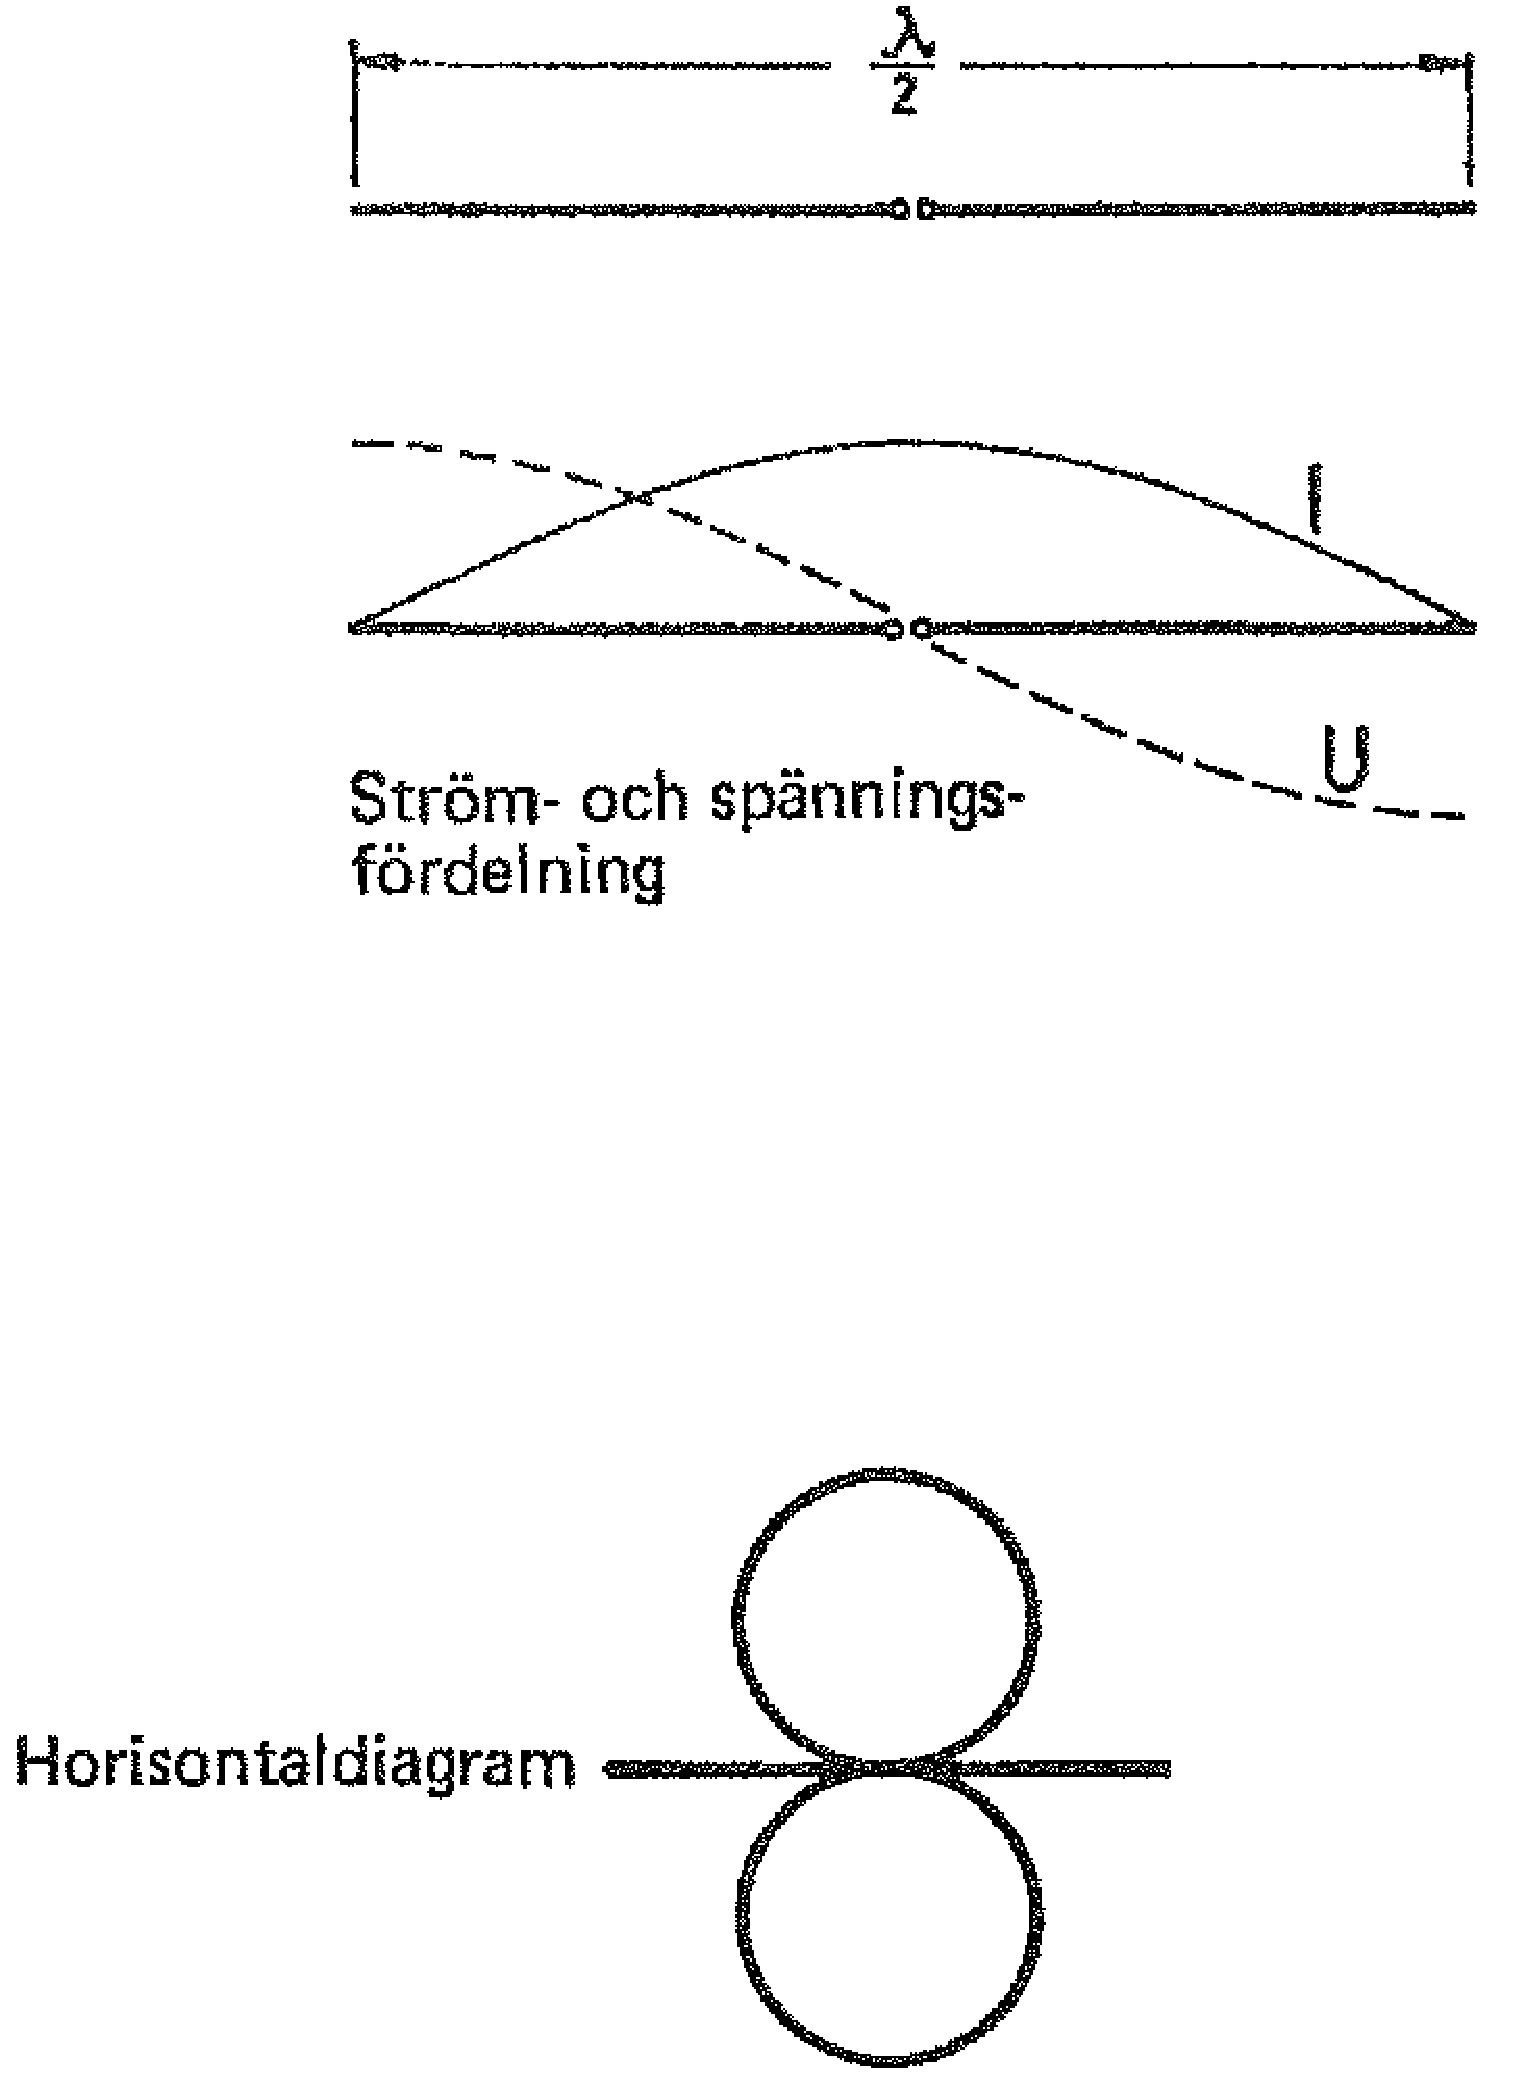
\includegraphics[width=0.5\textwidth]{images/cropped_pdfs/bild_2_6-01.pdf}
  \caption{Spänning och ström i en halvvågsantenn}
  \label{fig:bildII6-1}
\end{wrapfigure}

När en halvvågsantenn matas med HF-energi på grundfrekvensen, så uppstår en
stående våg med ett typiskt utseende.

Bild \ref{fig:bildII6-1} visar att i vardera änden av antennen uppnår spänningen
\(U\) ett maximum (en spänningsbuk), i mitten uppnår strömmen \(I\)
ett maximum (en strömbuk).
Antennen strålar mest där strömbuken finns.

Tag till exempel en 40~meter lång metalltråd som antenn.
Frekvensen för grundresonansen är ca 3,5~MHz, men den är även i resonans på de
harmoniska övertonerna (7, 14, 21, 28~MHz osv.).

Bild \ref{fig:bildII6-3} visar ström- och spänningsfördelningen på antennen vid
de respektive övertonerna.

För 80~m (3,5~MHz) är matningpunkten ett i spänningsminimum (en spänningsnod)
och ett strömmaximum (en strömbuk).
Strömmen är hög därför att matningspunkten har låg impedans.

Samma antenn på 40~m, 20~m, 15~m, 10~m (7, 14, 21, 28~MHz) har ett
spänningsmaximum (spänningsbuk) och ett strömminimum (strömnod) i
matningspunkten, som då har hög impedans.

Ur horisontaldiagrammet för antennen kan utläsas att ytterligare
strålningskäglor (strålningslober) utvecklas för varje överton i den
påmatade frekvensen.
Samtidigt blir strålningen alltmer till riktad längs med antennen.

\subsection{Impedansen i antennens matningspunkt}
\textbf{
HAREC a.\ref{HAREC.a.6.2.2}\label{myHAREC.a.6.2.2}
}
\index{impedans!antenn}
\index{antenn!impedans}
\index{halvvågsantenn}
\index{antenn!halvvågs}
\index{överton}

\begin{wrapfigure}{R}{0.5\textwidth}
  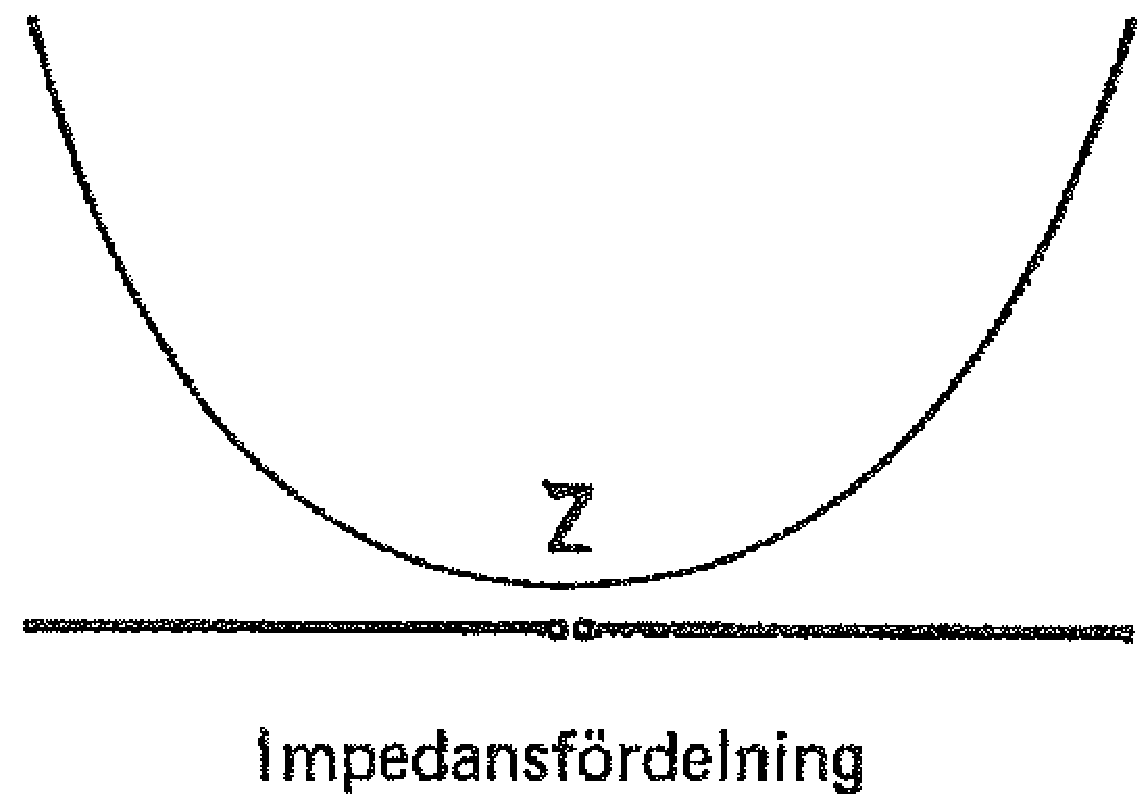
\includegraphics[width=0.5\textwidth]{images/cropped_pdfs/bild_2_6-02.pdf}
  \caption{Matningsimpedansen i en halvvågsantenn}
  \label{fig:bildII6-2}
\end{wrapfigure}

\begin{figure}
  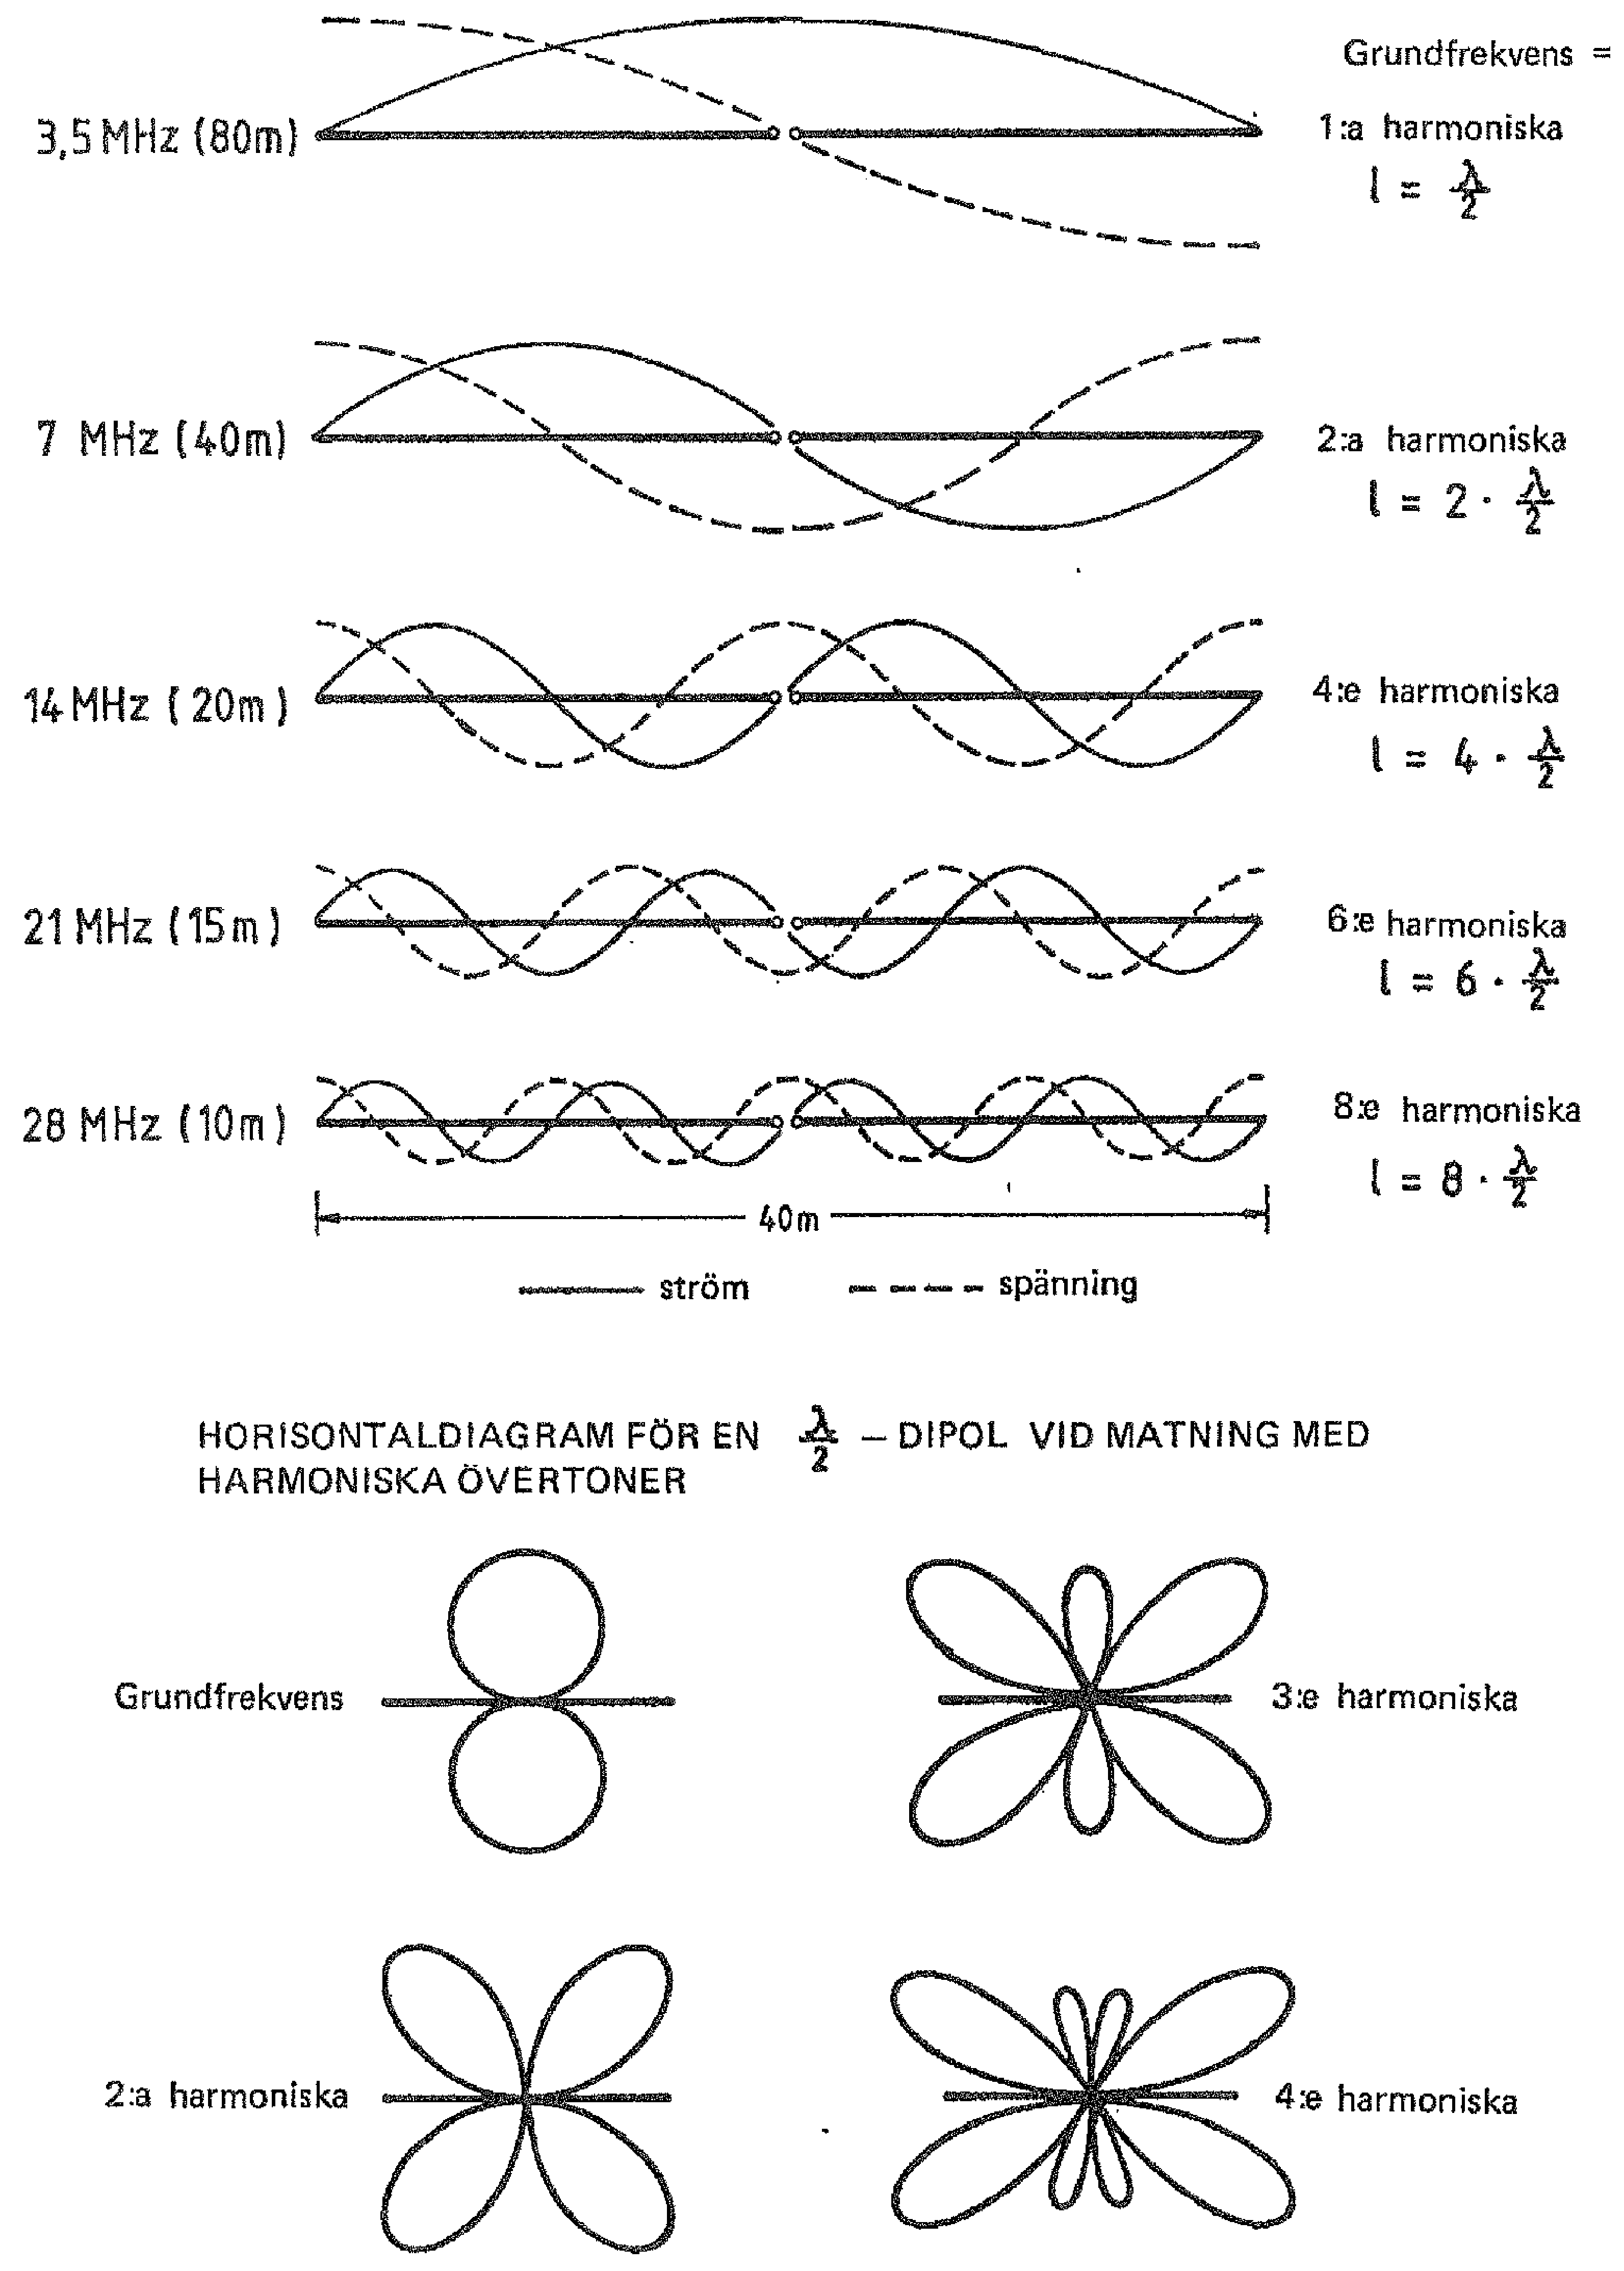
\includegraphics[width=\textwidth]{images/cropped_pdfs/bild_2_6-03.pdf}
  \caption{Halvvågsdipol matad med harmoniska övertoner}
  \label{fig:bildII6-3}
\end{figure}

Impedansen \(Z\) för varje punkt på en antenn kan beräknas med Ohms lag
\(Z = \frac{U}{I}\).

Bild \ref{fig:bildII6-2} visar matningsimpedansen i en halvvågsantenn.
På grundfrekvensen för en halvvågsantenn är impedansen \(Z\) i antennens
mittpunkt låg då spänningen är låg och strömmen hög i mittpunkten.
I halvvågsantennens yttre punkter är det tvärt om, impedansen är hög eftersom
strömmen är låg och spänningen är hög.

När antennen, mätt i våglängder, befinner sig mycket högt över jordytan, dvs.
utan nämnvärd påverkan från omgivningen är impedansen i mittpunkten 73~\(\Omega\)
på grundfrekvensen,.
I praktiken kan impedansen avvika mycket från detta värde.

Antenn och matningskabel måste vara impedansanpassade till varandra
för att det inte ska uppstå vågreflexion i anslutningen.

Märk, att halvvågsantennen är i resonans inte bara på grundtonen utan även på
övertoner.
För 2:a, 4:e etc. harmoniska övertonen har matningspunkten hög impedans.
Vid matning med en lågohmig koaxialkabel uppstår då en kraftig missanpassning i
anslutningen mellan antenn och kabel, vilket måste åtgärdas på något sätt.
Se avsnitt \ref{transmissionsledningar} i detta kapitel.

\subsubsection{Matningsimpedansen i några antenner}
\index{W3DZZ-antenn}
\index{antenn!W3DZZ}

Med W3DZZ-antennen (se avsnitt \ref{W3DZZ}) löses hjälpligt anpassningsproblemet
med mittmatade partier på 2:a harmoniska övertonen, dvs. dubbla
grundfrekvensen.
På 80- och 40~m-banden är antennens matningsimpedans ca 60~\(\Omega\) och på de
högre banden ca 100~\(\Omega\).
En kompromiss är att mata denna antenn med en 75~\(\Omega\)-kabel för att inte
få alltför stor missanpassning på något band.

\paragraph{Den omvikta dipolen (folded dipole):}
\index{omvikt dipol}
\index{antenn!omvikt dipol}
\index{folded dipol}
\index{antenn!folded dipol}

Matningsimpedansen är ca 240~\(\Omega\).
En bandkabel med impedansen 300~\(\Omega\) kan användas alternativt en
koaxialkabel med impedansen 50 eller 75~\(\Omega\) över en transformator med
impedansomsättningen 4:1.

\paragraph{Jordplanantennen (GP-antennen):}
\index{jordplanantenn}
\index{antenn!jordplan}
\index{GP-antenn}
\index{antenn!GP}

Matningsimpedansen är 30--60~\(\Omega\).
När jordplanets spröt inte riktas horisontellt, utan snett nedåt, erhålls en
matningsimpedans av 50~\(\Omega\), vilket passar bra för en koaxialkabel med
50~\(\Omega\) impedans.

\paragraph{Yagi- och Quad-antenner:}
\index{yagiantenn}
\index{Yagi-Uda}
\index{antenn!yagi}
\index{antenn!Yagi-Uda}
\index{quadantenn}
\index{antenn!Quad}

En anpassningsanordning för anslutning av 50~\(\Omega\) koaxialkabel ingår
oftast i fabriksgjorda riktantenner.
En 50~\(\Omega\) koaxialkabel kan då anslutas direkt till antennens matningspunkt.

\subsubsection{Reaktansen i en icke-resonant antenn}
\textbf{
HAREC a.\ref{HAREC.a.6.2.3}\label{myHAREC.a.6.2.3}
}
\index{reaktans!antenn}
\index{antenn!reaktans}

Den elektriska svängningskretsen behandlas i avsnitt \ref{oscillatorer}.
Där framställs svängningskretsens grundegenskaper resistans \(R\),
induktans \(L\) och kapacitans \(C\) som koncentrerade till komponenter kallade
resistor, induktor respektive kondensator.

Även en enkel tråd har dessa egenskaper, men fördelade över hela tråden.
Denna kan därför ses som ett stort antal komponenter, som tillsammans bildar en
svängningskrets, vilken naturligtvis kan fungera som antenn.

När antennen matas med växelström med samma frekvens som antennens
resonansfrekvens, så svänger antennen med minsta impedansen.
Resonansfallet kan i korthet beskrivas så att den induktiva och kapacitiva
reaktansen i antennen tar ut varandra medan resistansen kvarstår.

Impedansen är vektorsumman av resistansen och de kapacitiva och
induktiva reaktanserna.
I resonans är antennens impedans lika med resistansen, vilket är ett
specialfall.

Om sändningsfrekvensen är en annan än antennens resonansfrekvens, så händer
endera av följande:

När antennströmmen har lägre frekvens än antennens resonansfrekvens, så blir
den resulterande reaktansen negativ (kapacitiv), dvs. \(X_C\) är större
än \(X_L\).

När antennströmmen har högre frekvens än antennens resonansfrekvens,
så blir den resulterande reaktansen positiv (induktiv), dvs. \(X_L\)
är större än \(X_C\).

\subsection{Elektrisk ''förlängning'' och ''förkortning''}
\label{elektrisk förlängning}
\index{elektrisk förlängning}
\index{antenn!elektrisk förlängning}
\index{elektrisk förkortning}
\index{antenn!elektrisk förkortning}

\begin{wrapfigure}{R}{0.5\textwidth}
  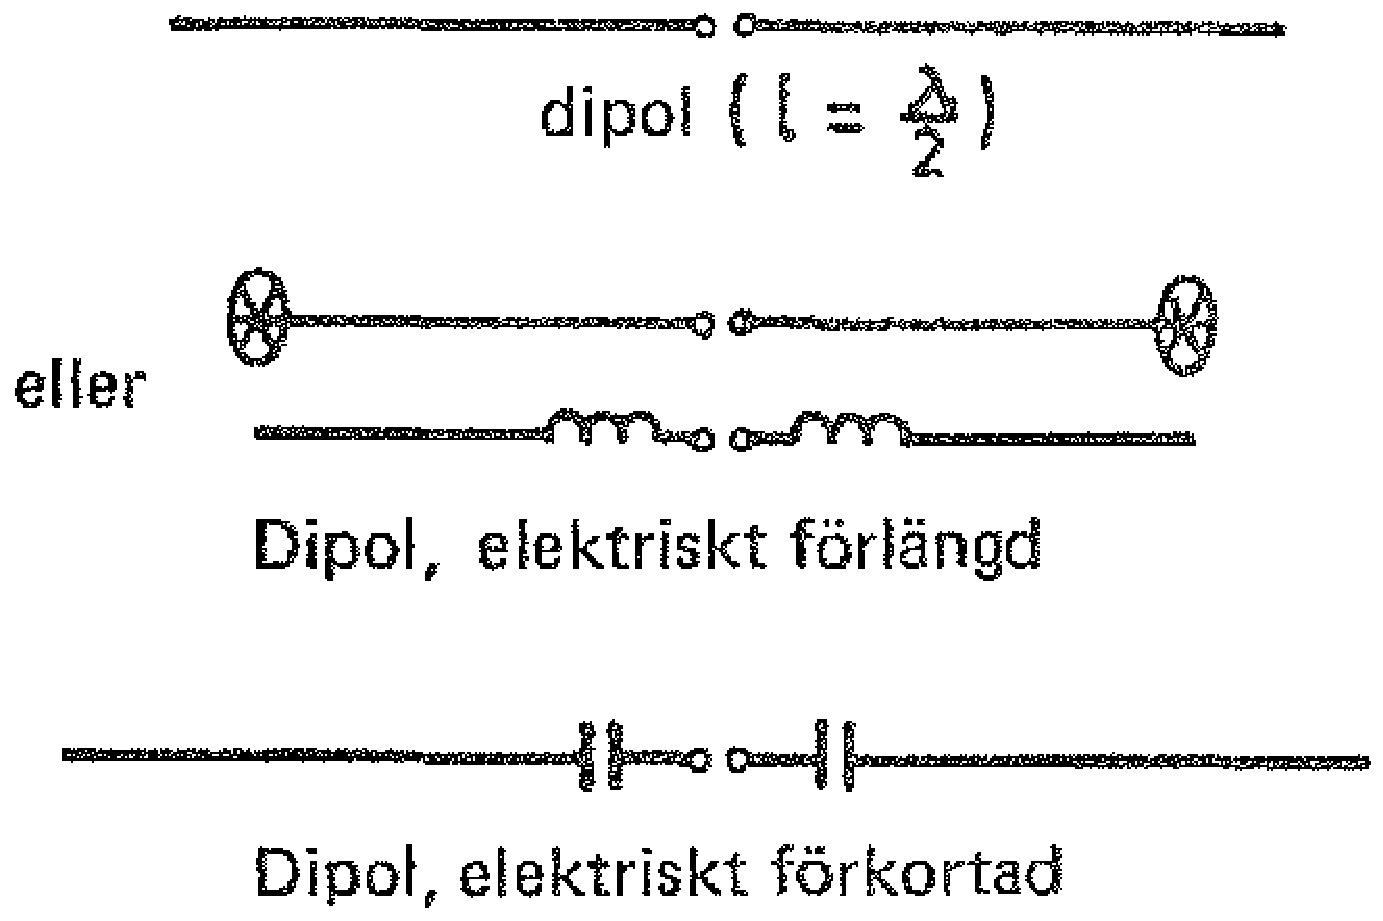
\includegraphics[width=0.5\textwidth]{images/cropped_pdfs/bild_2_6-04.pdf}
  \caption{Elektrisk förlängning och förkortning av antenner}
  \label{fig:bildII6-4}
\end{wrapfigure}

Om sändarfrekvensen, avviker mycket från antennens resonansfrekvens,
så kan reaktansen i antennen behöva elimineras eller åtminstone
minskas för en bättre impedansanpassning mellan antenn och matarledning.
Den enklaste åtgärden är då att försöka ändra antennlängden.

Om detta inte låter sig göras, så kan man i serie med en ''för kort''
antenn sätta in en induktor -- en så kallad elektrisk förlängning.
Om i motsatt fall antennen är ''för lång'', så kan man sätta in en
kondensator en så kallad elektrisk förkortning.
Bild \ref{fig:bildII6-4} visar elektriska förlängningar och förkortningar av
antenner.

Vid användningen av amatörradio ändras sändarfrekvensen ofta, varför
antennsystemet bör kunna stämmas av från marken/operatörsplatsen.
Då kan en antennkopplare med nödvändiga reaktiva komponenter behövas.
Se längre fram i kapitlet.

\subsection{Anpassning till sändarens impedans}
\textbf{
HAREC a.\ref{HAREC.a.5.3.7}\label{myHAREC.a.5.3.7}
}
\index{avstämningsanordning}
\index{match}
\index{sändare!match}
\index{impedansanpassning}
\index{sändare!impedansanpassning}
\index{\(\pi \)-filter}
\index{sändare!\(\pi \)-filter}
\index{ståendevåg}

Ett sändarslutsteg med elektronrör är vanligen utrustat med en
\emph{avstämningsanordning} (eng. \emph{matching network} och \emph{match})
vid HF-utgången.
Syftet är att kunna anpassa sändarens utgångsimpedans till impedansen i
antennledningen.
I moderna sändare består denna anordning mycket ofta av ett så kallat
\(\pi \)-filter, vars utgångsimpedans kan variera mellan ca 30--150~\(\Omega\).

Ett transistoriserat slutsteg är oftast utfört för en fast utgångsimpedans av
50~\(\Omega\) och är alltså i behov av en avstämningsanordning, om inte
antennsystemet inom vissa gränser håller samma impedans.
Toleransgränsen för felanpassning brukar vara ett SVF av storleksordningen 2:1
innan sändarens skyddskretsar automatiskt minskar uteffekten.

Vid lika impedans i sändarutgång, matarledning och antennanslutning
uppträder ingen stående våg på matarledningen och mesta möjliga effekt
överförs från sändaren till antennen.

\subsection{Antennens strålningsdiagram}
\index{strålningsdiagram}
\index{antenn!strålningdiagram}

\begin{figure}
  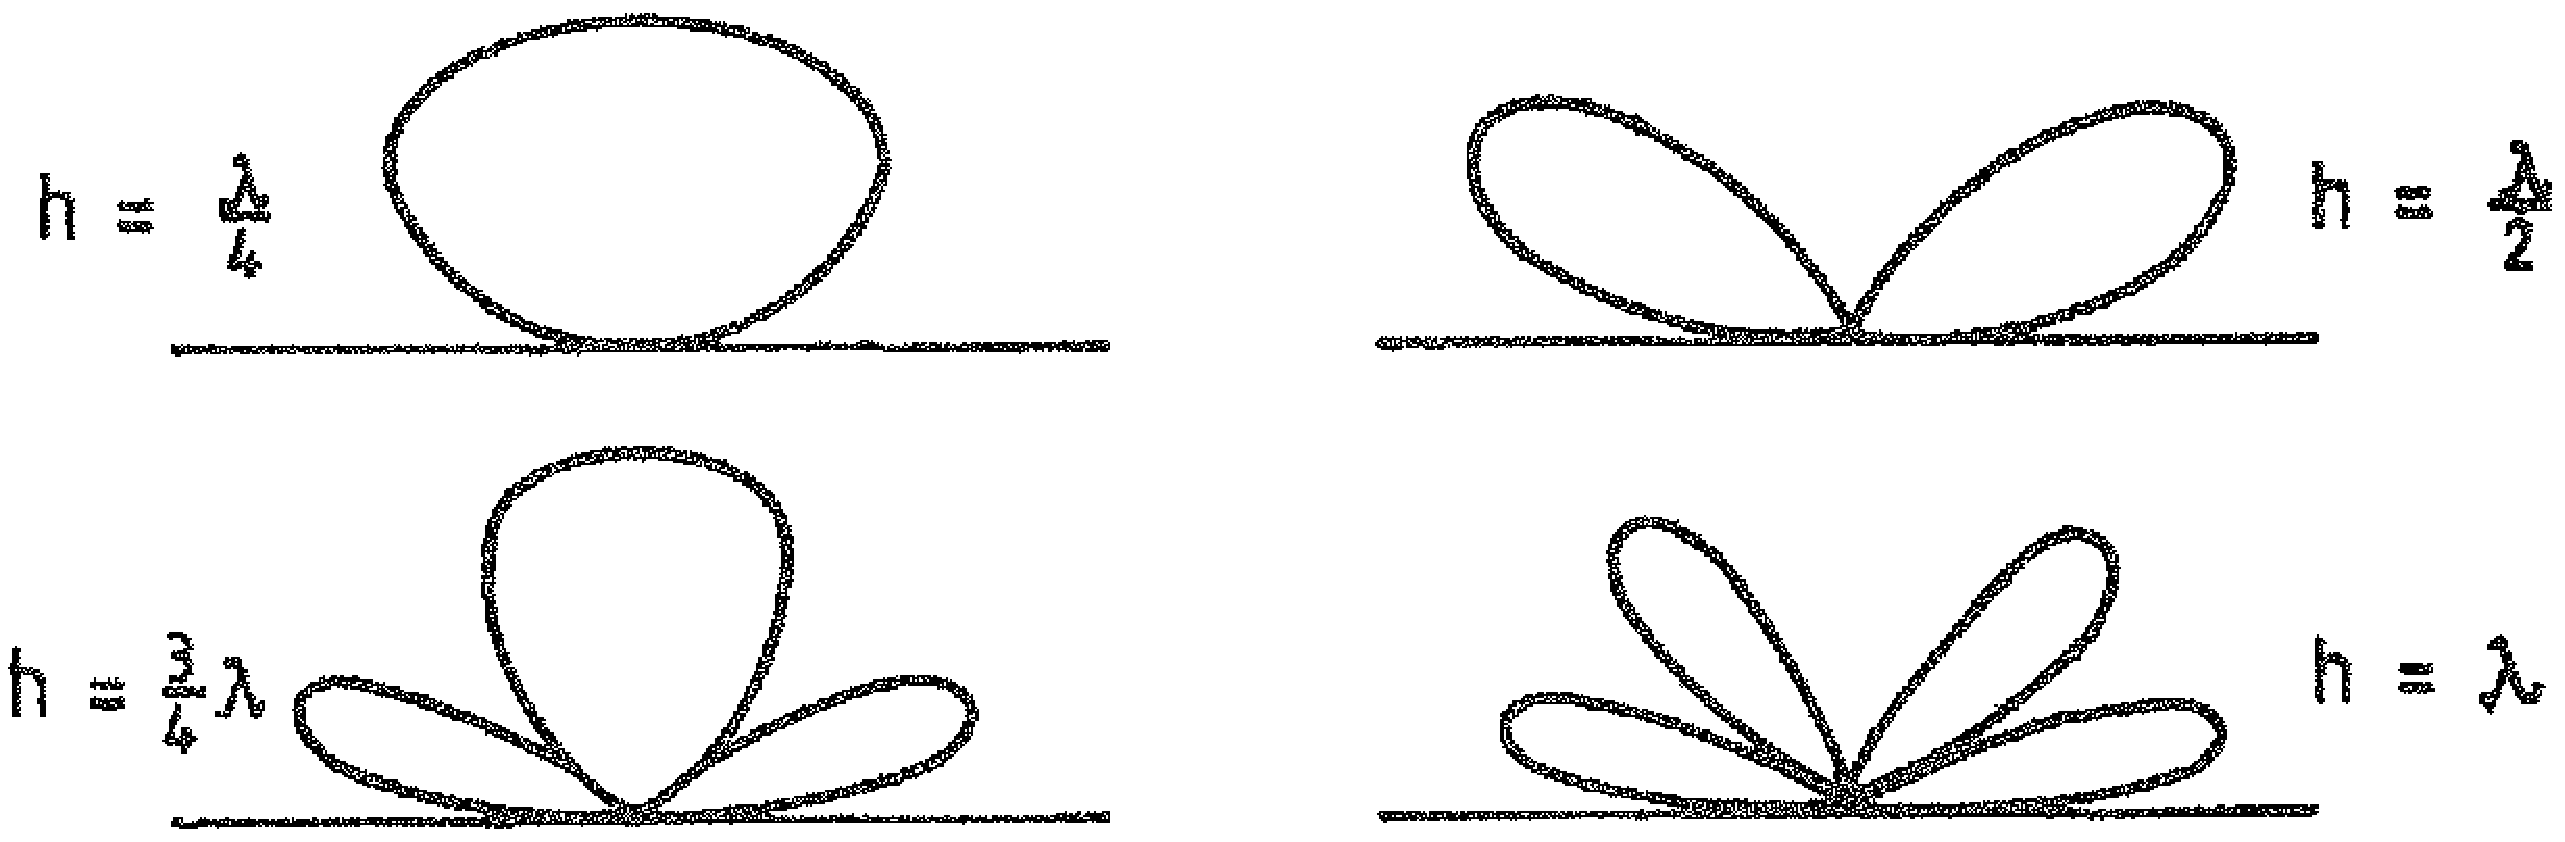
\includegraphics[width=\textwidth]{images/cropped_pdfs/bild_2_6-05.pdf}
  \caption{Vertikaldiagram för halvvågsantenn}
  \label{fig:bildII6-5}
\end{figure}

En antenns strålningsbild beskrivs bäst i tre dimensioner.
Bild \ref{fig:bildII6-3} visar bland annat ett horisontaldiagram för en
halvvågsantenn.

Bild \ref{fig:bildII6-5} visar strålningen i vertikalplanet som funktion av
antennhöjden för samma antenn.
Vertikaldiagrammet kan ha mycket olika utseende beroende på antennens utförande,
dess elektriska höjd över mark och omgivningens elektriska egenskaper.
För att överbrygga stora avstånd, måste antennen ha en flack utstrålning
relativt markplanet.

En horisontelit upphängd antenn med en längd av \(\lambda/2\) har övervägande
flack utstrålning när den placeras på en höjd av \(\lambda/2\), \(\lambda\),
\(3\lambda/2\), \(2\lambda\), osv. över mark.

När en horisontell antenn däremot placeras \(\lambda/4\), \(3\lambda/4\),
\(5\lambda/4\) osv. över mark, är utstrålningen övervägande vertikal, vilket
inte ska förväxlas med polarisationen, som i detta fall är horisontell.

Samma diagram gäller både för en sändar- och mottagarantenn. styrkan
på en utstrålad signal motsvaras av styrkan på mottagen signal.

\subsection{Antennvinst}
\textbf{
  HAREC a.\ref{HAREC.a.6.2.5}\label{myHAREC.a.6.2.5}
}
\index{antennvinst}
\index{antenn!antennvinst}
\index{antennförstärkning}
\index{antenn!antennförstärkning}
\index{isotropisk antenn}
\index{antenn!isotropisk}
\index{symbol!\(G_{ant}\) antennförstärkning}
\index{dBi isotropiskt gain}
\index{antenn!dBi isotropiskt gain}
\index{isotropisk förstärkning (dBi)}
\index{antenn!isotropiskt förstärkning (dBi)}
\index{dBd dipol gain}
\index{antenn!dBd dipol gain}
\index{dipol gain (dBd)}
\index{antenn!dipol gain (dBd)}

Med \emph{antennvinst} eller \emph{antennförstärkning} \(G_{ant}\) (eng.
\emph{antenna gain}) menas förhållandet mellan effekten \(P_t\) i
huvudstrålningsriktningen (framriktningen för en antenn med osymmetriskt
utstrålad effekt) och effekten från en definierad referensantenn.

Förmågan att ha högre antennförstärkning i en riktning i förhållande till andra
riktningar kallas för direktivitet (eng. \emph{antenna directivity}).

En referensantenn som tänks vara oändligt liten och som strålar med exakt
samma effekt \(P_t\) i alla riktningar kallas \emph{isotropisk antenn}.
En isotropisk antenn är emellertid endast teoretisk definierbar.

Med effekten \(P_i\) från den isotropiska antennen som referens blir
antennförstärkningen

\[G = 10 \log\frac{P_t}{P_i} \quad \text{[dBi]}\]

En i praktiken definierbar referens är halvvågsdipolen, vars
huvudstrålning är vinkelrätt ut från dipolen och runt omkring den.
Referenseffekten är då \(P_d\) och antennförstärkningen

\[G = 10 \log\frac{P_t}{P_d} \quad \text{[dBd] Bild \ref{fig:bildII6-6}}\]

Bild \ref{fig:bildII6-6} visar antennförstärkningen med dBd i effekt.

\begin{wrapfigure}{R}{0.5\textwidth}
  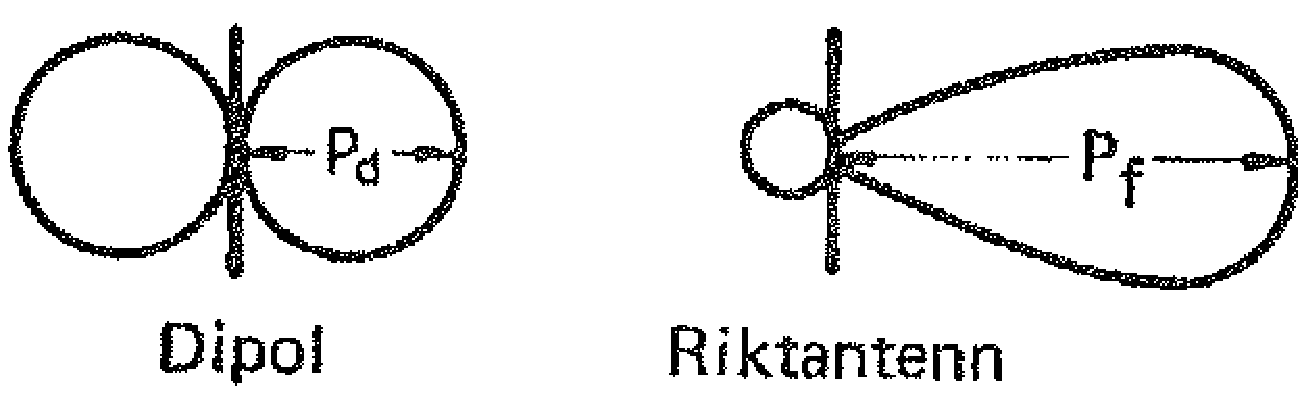
\includegraphics[width=0.5\textwidth]{images/cropped_pdfs/bild_2_6-06.pdf}
  \caption{Antennförstärkning dBd i effekt}
  \label{fig:bildII6-6}

  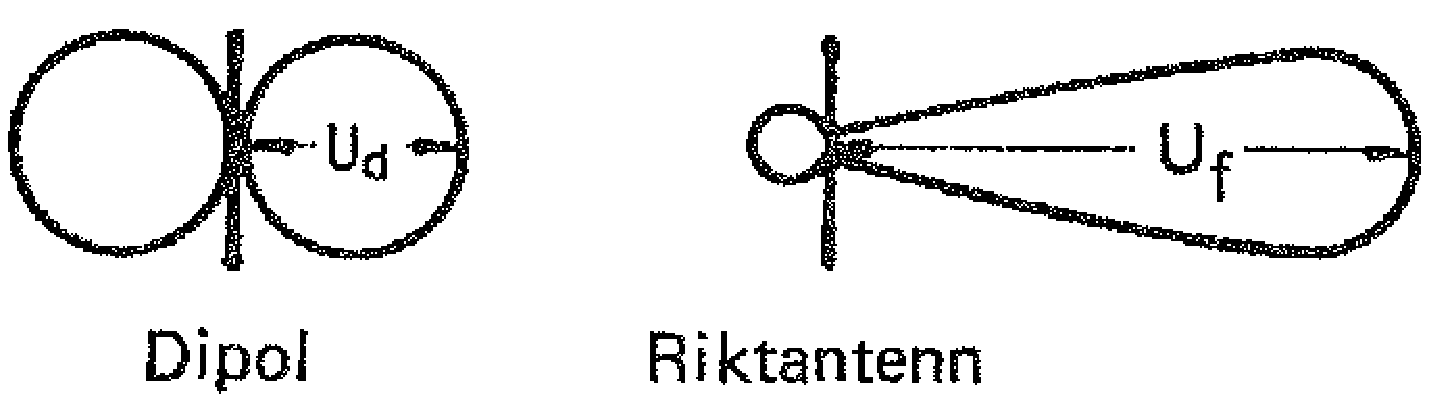
\includegraphics[width=0.5\textwidth]{images/cropped_pdfs/bild_2_6-07.pdf}
  \caption{Antennförstärkning dBd i spänning}
  \label{fig:bildII6-7}
\end{wrapfigure}

Antennförstärkning kan också definieras som förhållandet mellan den elektriska
fältstyrkan uf i huvudstrålningsriktningen och referensfältstyrkan (dipol).

Jämfört med \(\lambda/2\)-dipol är antennförstärkningen

\[G = 20 \log\frac{U_t}{U_d} \quad \text{[dBd] Bild \ref{fig:bildII6-7}}\]

Man använder uttrycket dBi när antennförstärkningen anges i förhållande till
en isotrop antenn och dBd i förhållande till en halvvågsantenn.
Se kapitel \ref{decibel} om decibelbegreppet.

\textbf{Exempel på beräkning av antennförstärkning:}

\begin{align*}
  U_f &= 40\text{ \(\mu V\)} \quad U_d = 20\text{ \(\mu V\)} \quad G =\ ? \\
  G &= 20 \log\frac{U_f}{U_d} = 20 \log\frac{40}{20} \\
  &= 20 \log 2 = 20\cdot 0.3 = 6 \quad \text{[dBd]} \\
\end{align*}

6~dB antennförstärkning motsvarar en fördubblad fältstyrka [V/m], dvs.
1~S-enhets ökning vid den mottagande stationen, liksom att 6~dB
antennförstärkning motsvarar en 4~dubblad sändareffekt \(\mathrm{[W/m^2]}\).

Ungefärlig antennförstärkning för olika antenner med en isotrop antenn som
referens:

\begin{tabular}{l|ll|ll}
  & \multicolumn{2}{l|}{\(\lambda/2\)-dipol} &
  \multicolumn{2}{l}{Isotrop} \\
  \hline
  Isotrop antenn       & -2,1 & dBd & 0   & dBi \\
  GP, \(\lambda/4\)    & -1,8 & dBd & 0,3 & dBi \\
  Dipol, \(\lambda/2\) & 0    & dBd & 2,1 & dBi \\
  GP, \(5/8\lambda\)   & 1,2  & dBd & 3,3 & dBi \\
  & & & & \\
  Dipol, \(1/1\lambda\) & 1,8 & dBd & 3,9  & dBi \\
  2-elements yagi       & 5   & dBd & 7,1  & dBi \\
  2-elements quad       & 6   & dBd & 8    & dBi \\
  3-elements yagi       & 8   & dBd & 10,1 & dBi \\
\end{tabular}

Antenner har förluster, det gör att olika antenner kan ha olika
effektivitet, därför finns måttet \emph{antenneffektivitet}
(eng. \emph{antenna efficiency}) \(\eta\) som beror på relationen mellan
utstrålningsresistansen \(R_R\) och förlustresistansen \(R_L\)

\[\eta = \frac{R_R}{R_R+R_L}\]

Antennens effektivitet, verkningsgrad, kan även beräknas med hjälp av antennens
förlusteffekt och den tillförda effekten.
Observera att verkningsgraden för en antenn alltid är mindre än 1 då det är lätt
att förväxla de olika effekterna i beräkningen.

\subsection{Effektivt utstrålad effekt}
\textbf{
HAREC a.\ref{HAREC.a.6.2.7}\label{myHAREC.a.6.2.7}
}
\index{effektivt utstrålad effekt (ERP)}
\index{antenn!effektivt utstrålad effekt (ERP)}
\index{Effective Radiated Power (ERP)}
\index{antenn!Effective Radiated Power (ERP)}
\index{ERP}
\index{antenn!ERP}
\index{ekvivalent isotropiskt utstrålad effekt (EIRP)}
\index{antenn!ekvivalent isotropiskt utstrålad effekt (EIRP)}
\index{Equivalent Isotropically Radiated Power (EIRP)}
\index{antenn!Equivalent Isotropically Radiated Power (EIRP)}
\index{EIRP}
\index{antenn!EIRP}

Effektivt utstrålad effekt (ERP) (eng. \emph{effective radiated power}) är den
effekt som sändarantennen strålar ut i sin bästa strålningriktning.
ERP beräknas som den effekt som tillförs själva antennen, multiplicerat med
antennvinsten relativt en halvvågsdipol.
Förlusterna på vägen från sändaren till antennen räknas bort före beräkningen av
ERP.

Ekvivalent isotropiskt utstrålad effekt (EIRP)
(eng. \emph{Equivalent isotropically radiated power}).
EIRP beräknas relativt en teoretisk antenn (\emph{isotropisk antenn}) som
strålar lika mycket i alla riktningar.
Vid beräkningen används den effekt som tillförs själva antennen, multiplicerat
med antennvinsten relativt en isotrop.
På samma sätt som vid beräkningen av ERP ska förlusterna på vägen från sändaren
till antennen räknas bort före beräkningen av EIRP.

\subsection{Fram/backförhållande (antennvinst)}
\textbf{
HAREC a.\ref{HAREC.a.6.2.8}\label{myHAREC.a.6.2.8}
}
\index{fram/backförhållande}
\index{antenn!fram/backförhållande}

Med fram/backförhållande (F/B) för en riktantenn menas förhållandet mellan den
utstrålade effekten i framriktningen \(P_f\) och effekten i backriktningen
\(P_b\).

\[ F/B = 10 \log\frac{P_f}{P_b} \quad \text{[dB]} \]

\begin{wrapfigure}{R}{0.5\textwidth}
  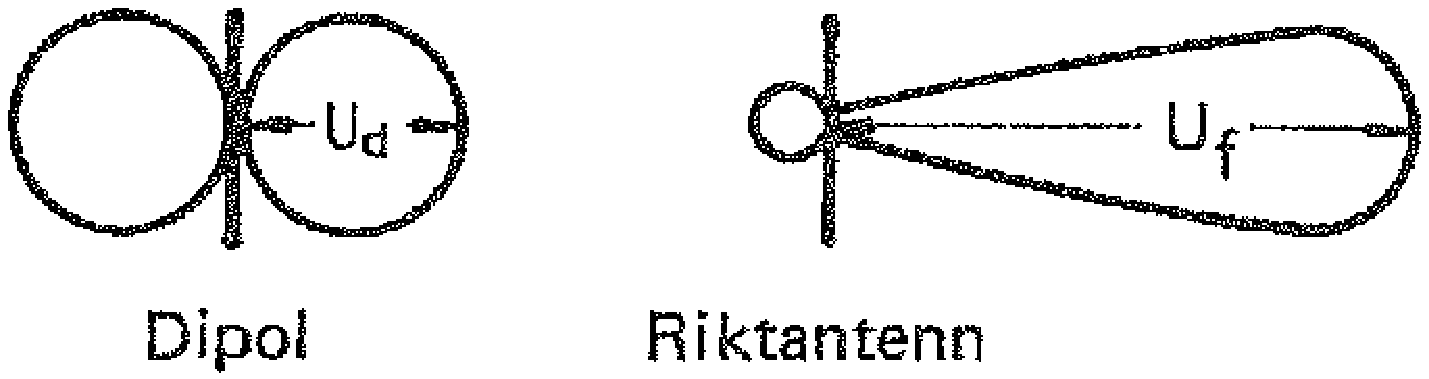
\includegraphics[width=0.5\textwidth]{images/cropped_pdfs/bild_2_6-08.pdf}
  \caption{F/B-förhållande i effekt}
  \label{fig:bildII6-8}
\end{wrapfigure}

Fram/backförhållandet kan också definieras som förhållandet mellan elektriska
fältstyrkan \(U_f\) i framriktningen och referensfältstyrkan \(U_b\) i
backriktningen

\[ F/B = 20 \log\frac{U_f}{U_b} \quad \text{[dB]} \]

\begin{wrapfigure}{R}{0.5\textwidth}
  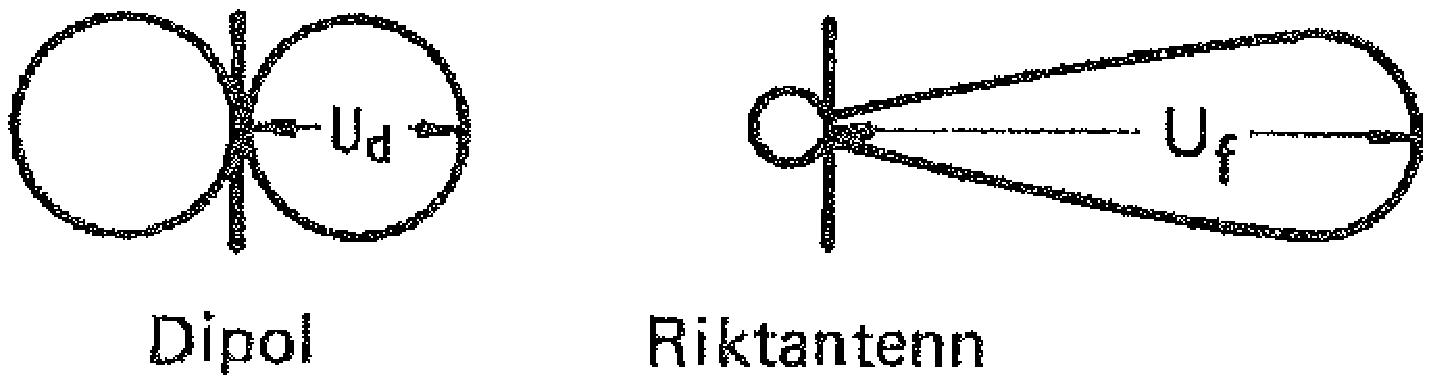
\includegraphics[width=0.5\textwidth]{images/cropped_pdfs/bild_2_6-09.pdf}
  \caption{F/B-förhållande i spänning}
  \label{fig:bildII6-9}
\end{wrapfigure}

\textbf{Exempel 1:}

\begin{align*}
  U_f &= 40 \text{ \(\mu V\)} \quad U_b = 4\text{ \(\mu V\)} \quad F/B =\ ? \\
  F/B &= 20 \log\frac{U_f}{U_b} = 20 \log\frac{40}{4} \\
  &= 20 \log 10 = 20 \cdot 1 = 20 \quad \text{[dB]} \\
\end{align*}

\(F/B = 20\) dB betyder att fältstyrkan \(U_f\) i huvudriktningen är
10 gånger så hög som fältstyrkan i backriktningen \(U_b\).

\textbf{Exempel 2:}

\begin{align*}
  U_f &= 15 \text{ \(\mu V\)} \quad U_b = 15\text{ \(\mu V\)} \quad F/B =\ ? \\
  F/B &= 20 \log\frac{U_f}{U_b} = 20 \log\frac{15}{15} \\
  &= 20 \log 1 = 20 \cdot 0 = 0 \quad \text{[dB]} \\
\end{align*}

\(F/B = 0\) dB betyder att \(U_f = U_b\), dvs. att fältstyrkorna i
fram- och backriktning är lika stora, vilket inträffar för en dipol.

\subsection{Halvvärdesbredd}
\index{halvvärdesbredd}
\index{antenn!halvvärdesbredd}

Studera diagrammet för den horisontella strålningen från en riktantenn.

Antennen avger sin största utstrålade effekt \(P_f\) i huvudriktningen.
Effekten avtar utanför huvudriktningen.
Fältstyrkan \(U_f\) förhåller sig på liknande sätt.

Med effekthalvvärdesbredd menas den vinkel inom vilken nyttoeffekten
är minst hälften så stor som i huvudriktningen.
Bild \ref{fig:bildII6-10} visar halvvärdesbredder.

\begin{gather*}
  \text{Observera, att } \frac{P_f}{2} \text{ motsvarar }
  \sqrt{\frac{1}{2}}U_f \\
  ( \approx 0,7 U_f \text{ motsvarande 3 dB })
\end{gather*}

Med spänningshalvvärdesbredd menas den vinkel inom vilken spänningen
(fältstyrkan) är minst hälften så stor som den största nyttospänningen \(U_f\).
Spänningshalvvärdesbredden för en dipol är ungefär 90\degree.

\begin{figure}
  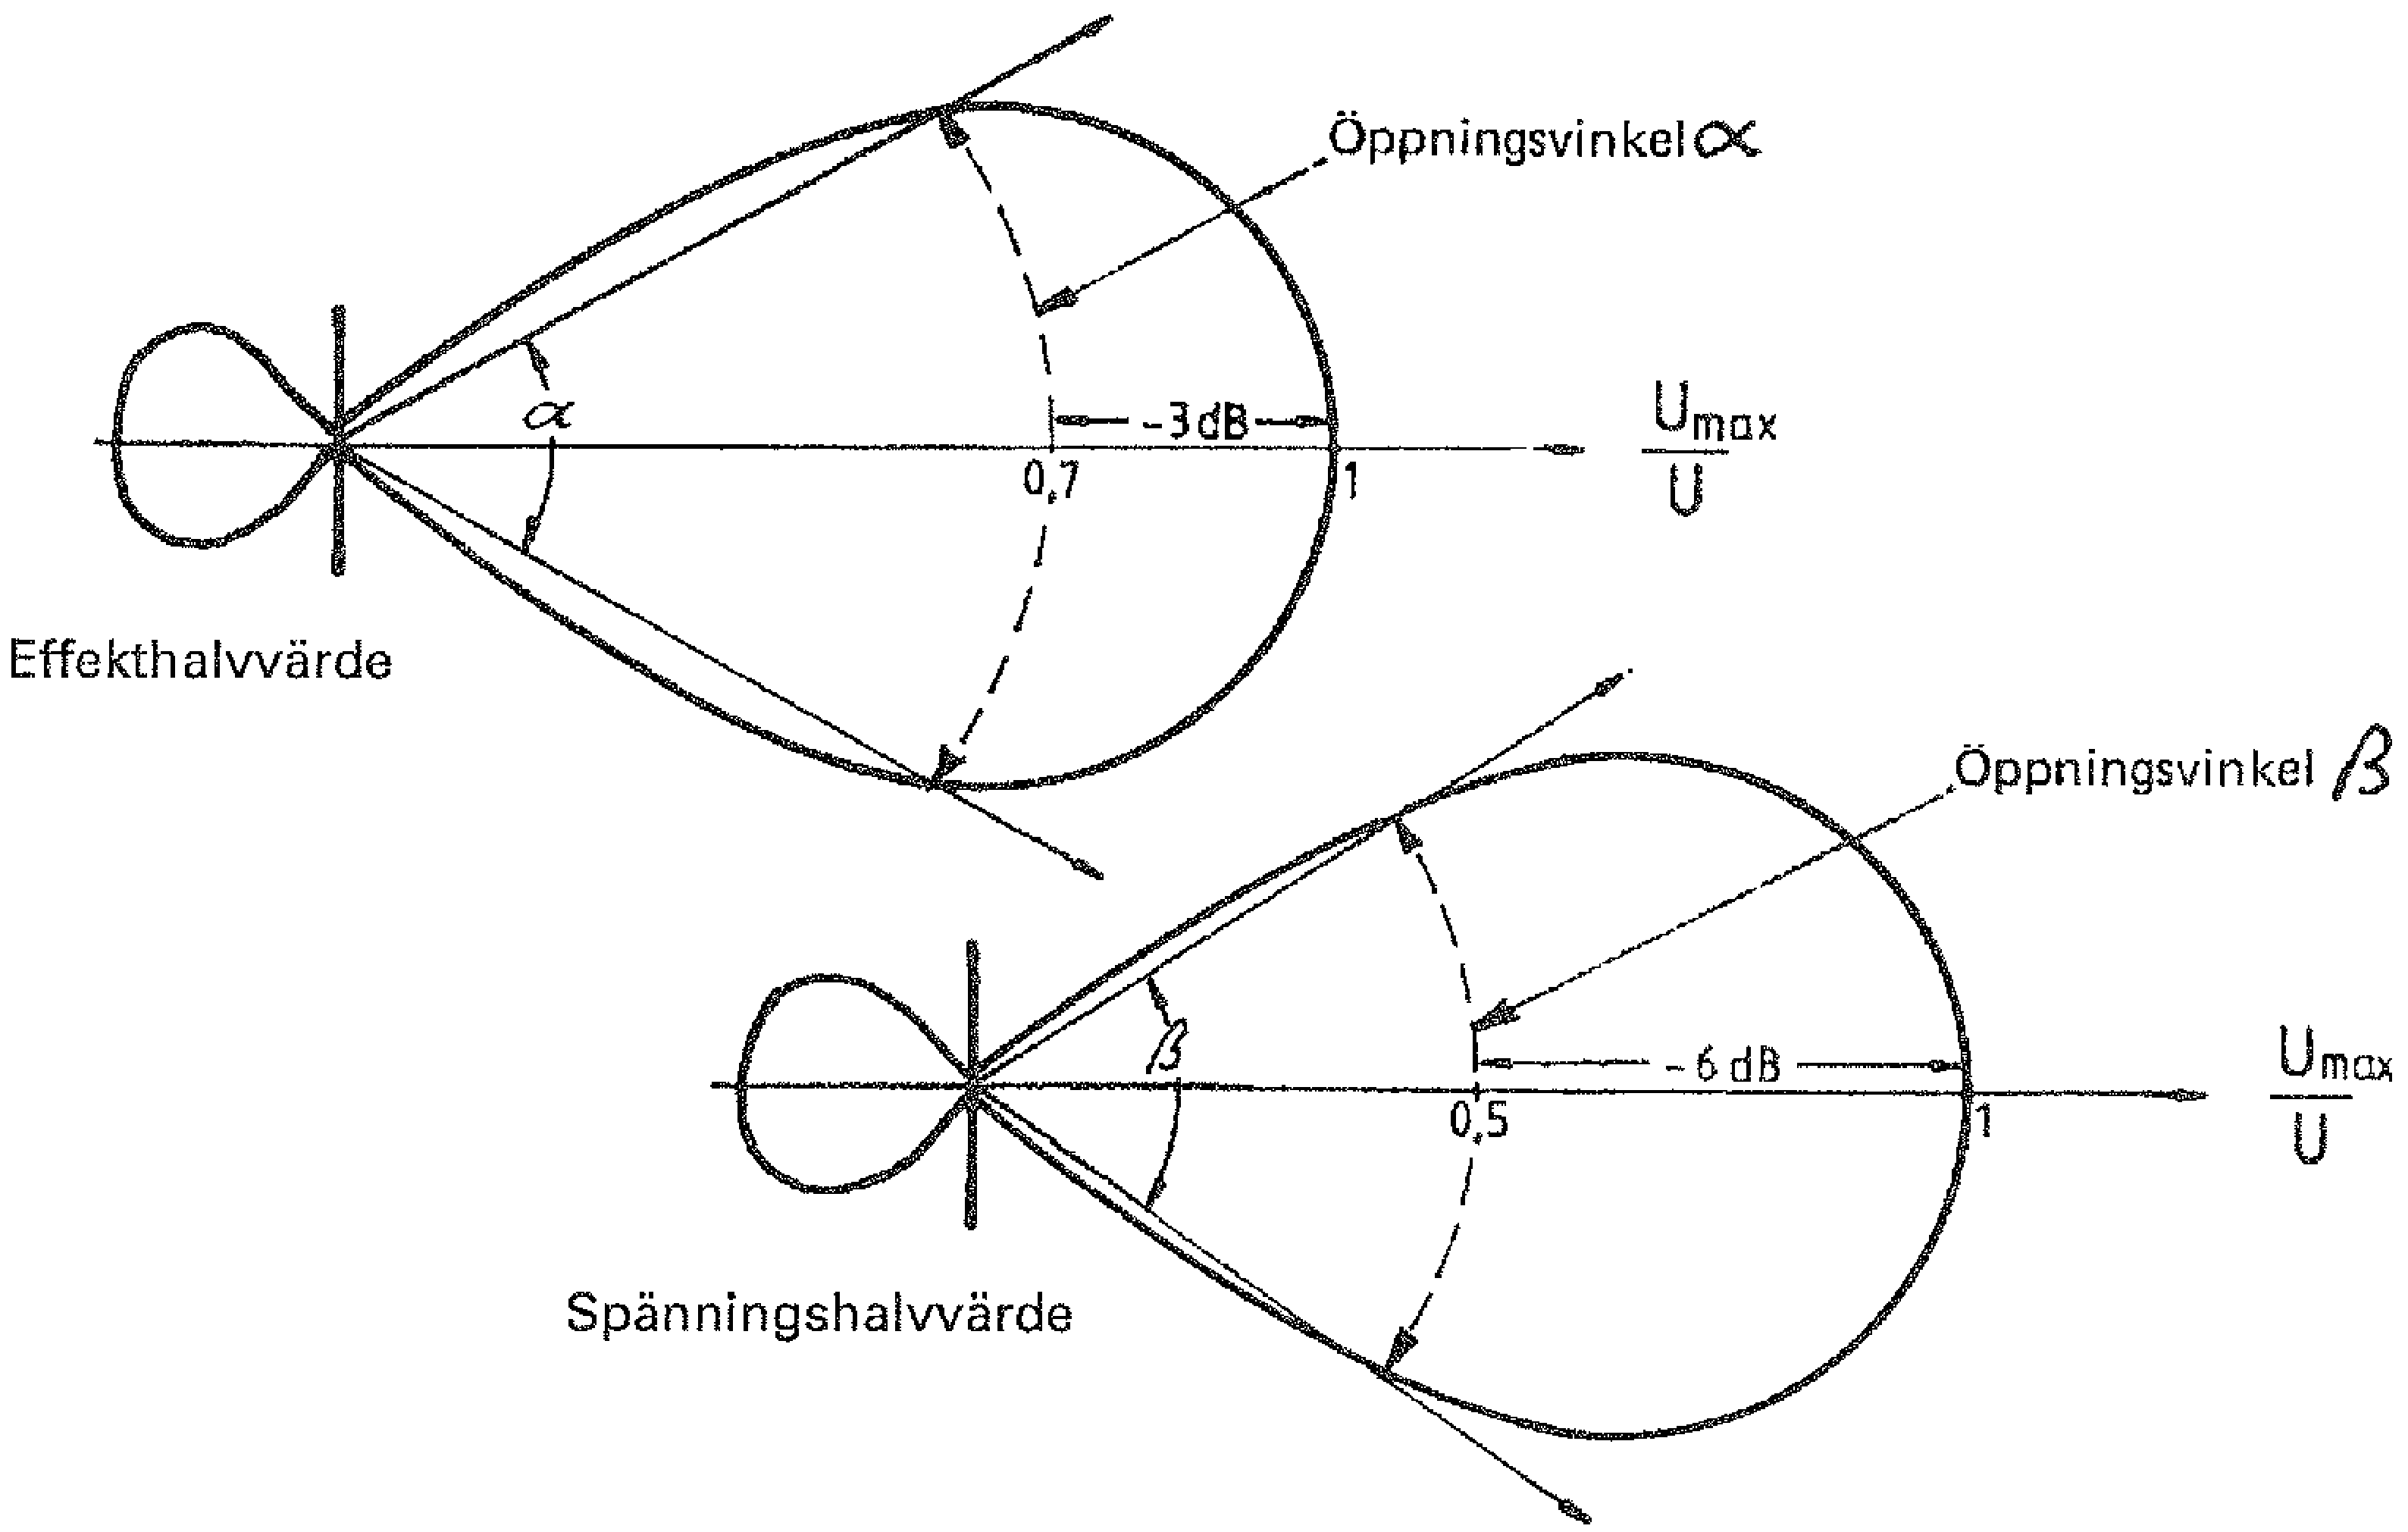
\includegraphics[width=\textwidth]{images/cropped_pdfs/bild_2_6-10.pdf}
  \caption{Halvvärdesbredder}
  \label{fig:bildII6-10}
\end{figure}

\subsection{Antennarea}
\textbf{
HAREC a.\ref{HAREC.a.6.2.6}\label{myHAREC.a.6.2.6}
}

\emph{Antennarea} (eng. \emph{capture area}) är den area som parabolantenner
och horn har.
Antenngainet (G) beror antennarean (\(A_{phy}\)), effektiviteten (\(e_a\)) och
våglängden (\(\lambda\)) enligt

\[ G = \frac{4\pi A_{phy}e_a}{\lambda^2} \]
9
